\chapter{Related Work}
\label{chap:relatedwork}
\numberwithin{equation}{chapter}
The concept of web crawling dates back to the early 1990s when the World Wide Web was still in its infancy.

WebCrawler, created by Brian Pinkerton in 1994, is considered the first true web crawler-powered search engine. While some may claim that title for Wandex is due to its potential, it was never designed to be used in this way. Wandex lacked some critical features to make it a general-purpose search engine.

One of the major innovations of WebCrawler was its full-text searchability. This ability made it popular and highly functional. It continues to operate as a search engine, although not as popular as Google, Yahoo, Bing, Yandex, or Baidu.

Modern web crawlers face many challenges and complexities, such as dynamic content, user interaction, authentication, robots.txt files, and ethical issues. Some examples of modern web crawlers are Googlebot, Bingbot, and Internet Archive

\section{Web crawlers list}
Web crawlers have evolved during the last few decades, with different designs and implementations to crawl and index the internet. Below is an enumeration of some of the architectural designs utilized in the development of all-encompassing web crawlers [3]:


\begin{itemize}
  \item RBSE [Eic94] Considered as one of the first Web crawlers to be published. Made of two components: the first component,
“spider”, uses a queue in a database. The second component, “mite”, is a modified browser that downloads the pages from the Web.
  \item WebCrawler [Pin94]  The initial publicly accessible full-text index of a specific portion of the World Wide Web was established. The approach involved leveraging lib-WWW for page downloads and employing an additional tool to parse and arrange URLs, ensuring a breadth-first approach to navigating the web graph.
  \item World Wide Web Worm [McB94] was a crawler designed to construct a basic index comprising document titles and corresponding URLs. This index could be queried by utilising the grep command in the UNIX operating system.
  \item Google Crawler [BP98] Google has been the market's dominant search engine for the last few decades. In March 2023, Google’s global market share was 85.53% [4].
The crawler was integrated with the indexing, and since this thesis has some similarity with the Google search engine design, we will explain this in-depth in the ext subsection [Google architecture]
  \item Ubicrawler [BCSV04] Is a Java-based distributed crawler with no central process and several identical “agents”. The crawler is implemented to provide high scalability and be tolerant of failures.
\end{itemize}



\section{High Level Google Architecture}

The Google search engine's design gives a good overview of the essential components to create a scalable search engine. Hence, it is a great starting point for any search engine research; we will explain it in this section. Most code written in the Google search engine was implemented in C or C++ for efficiency and because it can run on either Solaris or Linux [2]. Google uses distributed crawlers to download internet web pages. The URLserver keeps a list of the available found URLs that need to be crawled by the crawlers. URLserver acts as a load balancer that sends the URLs to the following free crawler. Afterwards, the crawlers download the documents needed from the page, associate a unique ID for this page called docID, and then the page's content are stored in Soreservers. Storeservers then compress the pages and save them on a repository. The indexer component then uncompresses the pages and parses them. Each document is then converted into a set of words called hits. The hits represent the word and its position in the document. Afterwards, the indexer distributes those hits into barrels. Moreover, the indexer collects links found in the crawled page and stores them in the anchor's file. The anchors' file contains the links and their relationship with each other [2].


\begin{figure}[h]	
     \centering
     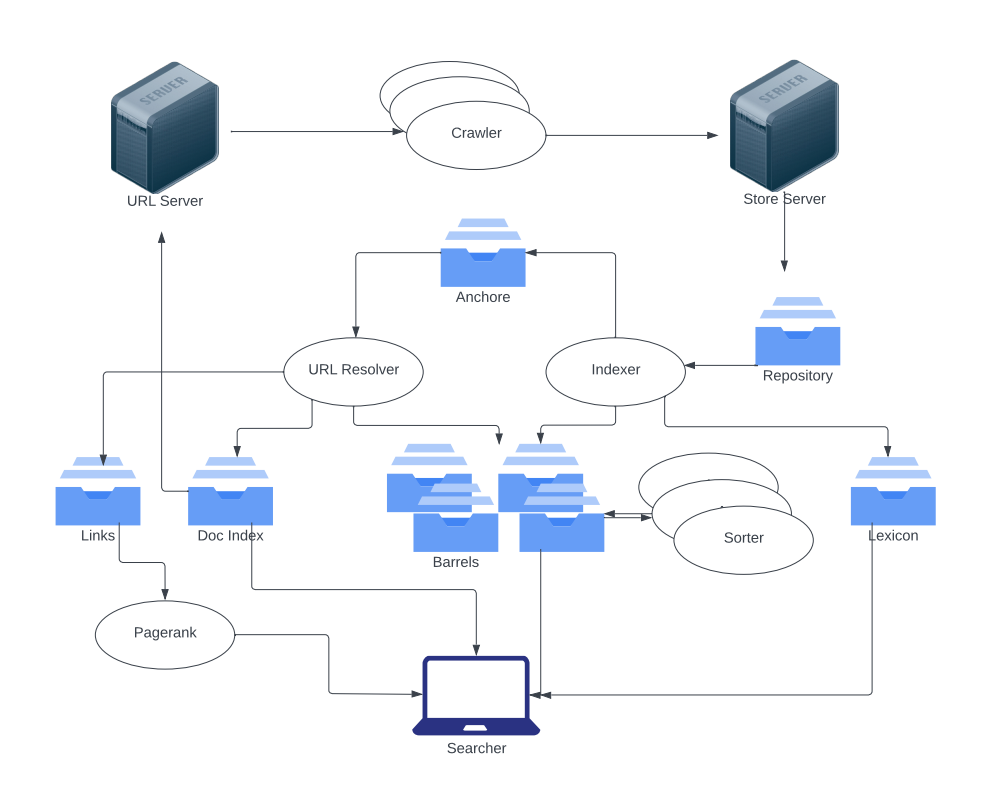
\includegraphics[width=10cm]{images/google_arch.png}
     \caption{High level view of Google web crawlers archeticture.}
     \label{fig:google-arch}
\end{figure}

The URLresolver reads the links from the anchors' file and converts the relative URLs into absolute URLs. The URLs are then assigned to their docID. The links database saves pairs of docIDs that will be used to compute PageRanks for all the documents. 

Initially organized by docID, the barrels are then rearranged by the sorter based on wordID. This process generates an inverted index. Moreover, the sorter generates a list of wordIDs and corresponding offsets within the inverted index. 

\section{User Friendly Crawlers}
Since this thesis also focuses on providing a friendly user interface to configure the search engine, it is advisable to look at the existing tools in the market. Although there are plenty of tools to parse the content of the internet without programming knowledge, two of the most well-known software are Octoparse and ParseHub. Since ParseHub has a free tier to test it and it supports Linux, I decided to go with it to evaluate my crawler and collect some ideas on how they approach the different challenges with configuring how to use the crawler for various websites. 

ParseHub is a user-friendly option well suited for users who want a straightforward User Interface tool to parse information from a specific website on the internet. It operates as a desktop application, catering to multiple platforms, including Linux, Windows and Mac OS X. Comparable to Octoparse, ParseHub adeptly handles intricate web scraping tasks outlined earlier. Despite its aspiration for simplicity in web scraping, users with particular technical understanding may need to delve into its more advanced features and grasp their intricacies [7].
